%% TODO: aspect ratio
\documentclass[aspectratio=169,dvipsnames]{beamer}

%% \usepackage{amssymb,amsmath,amsthm,latexsym}
%% \usepackage{url,hyperref}
\usepackage{multirow}           % \multirow, \multicolumn
\usepackage{nccmath}           % fleqn environment
\usepackage{mathpartir}        % \mathpar, \infer
\usepackage{booktabs}           % \midrule
%% \usepackage{colonequals}
\usepackage{tikz,tikz-cd}      % Hasse & commutative diagrams.
\usepackage{accents}           % \underaccent
\usepackage{pdfpages}           % \includepdf
\usepackage{mathtools}          % \dblcolon, vertically centered colon
%% \usepackage{pgfplots}\pgfplotsset{compat=1.5} % the perf graph
\usepackage{censor}             % \censor
\usepackage{array}              % alignment options in tabular
\usepackage{pbox}               % \pbox
\usepackage[normalem]{ulem}     % \sout

\mathtoolsset{centercolon} % not sure this works w/ Euler

\usepackage{iftex}
\ifPDFTeX\PassOptionsToPackage{spacing=true,tracking=true,letterspace=40,}{microtype}\else\fi
\usepackage{microtype}
\frenchspacing


%% Format fiddling.
\linespread{1.0608}
\def\arraystretch{1.05}

\let\olditemize\itemize
\renewcommand\itemize{\olditemize\setlength\itemsep{1ex}}

\colorlet{standout}{Orange!10!Red!75!black}
\newcommand\standout{\color{standout}}

\setbeamertemplate{navigation symbols}{}
%% TODO: figure out how to get this to work
\colorlet{bgcolor}{yellow!6!white}
%\setbeamercolor{background canvas}{bg=bgcolor}

\setbeamertemplate{footline}[frame number]
\setbeamerfont{footline}{size=\small,}
\setbeamerfont{frametitle}{shape=\scshape}
\setbeamercolor{frametitle}{fg=standout}
%\setbeamertemplate{footline}{\hfil\insertpagenumber\vspace{2ex}}
%% \setbeamerfont{headline}{size=\scriptsize}
%% \setbeamertemplate{headline}{\vspace{2ex}\hfill\insertpagenumber\hspace*{2ex}}


%% font fiddling
\usepackage[LY1,OT1,T1]{fontenc}
\ifPDFTeX\else\usepackage[no-math]{fontspec}\fi
\usefonttheme{professionalfonts}
\renewcommand{\familydefault}{\rmdefault}

%\usepackage[scaled=0.9543]{XCharter}
%\usepackage[llscale=1.0699300699300702,scale=1.0699300699300702,p,mono=false]{libertine}
%% \usepackage[semibold,scaled=0.9663]{sourceserifpro}
%% \usepackage[osf,semibold,scaled=0.9663]{sourcesanspro}
%% \usepackage[scaled=1.00438,varqu,var0]{inconsolata}

\usepackage{fontchoice}
\providecommand\displayfamily\rmfamily
\setmonofont{inconsolata}[Scale=MatchLowercase,Scale=1.00438,]

\usepackage{eulervm}
\usepackage[bb=boondox]{mathalfa} % or bb=ams
%\usepackage[euler-digits]{eulervm}


%% ===== COMMANDS =====
\providecommand\strong[1]{{\bfseries#1}}
\newcommand\textsfit[1]{\textsf{\itshape#1}}

\newcommand\N{\mathbb{N}}
\newcommand\x\times
\providecommand\G{}\renewcommand\G\Gamma
\newcommand\D\Delta
\newcommand\fn{\ensuremath{\lambda}}
\newcommand\isa{\hspace{.1em}:\hspace{.1em}}
\newcommand\fnof[1]{\fn{#1}.\;}
\newcommand\fa[1]{(\forall {#1})\ }
\newcommand\iso{{\texorpdfstring{\ensuremath{\square}}{box}}}
\newcommand\desugars{\,\xrightarrow{\textsf{desugars}}\,}

\newcommand{\setfor}[2]{\{{#1} \mathrel{|} {#2}\}}

\newcommand\kw\textbf
\newcommand\n\textit
\newcommand\tpname\text
%\newcommand\kw[1]{\textsfit{#1}}\newcommand\n\textsfit\newcommand\tpname\textsf
\renewcommand\c\textsf

\newcommand\tset{\tpname{set}\,}
\newcommand\tmap[2]{\tpname{map}\,(#1,#2)}
\newcommand\tbool{\tpname{bool}}
\newcommand\tunit{\ensuremath{1}}
\newcommand\tnode{\tpname{node}}
%\newcommand\mto{\overset{\textsf{\Large +}}{\to}}
\newcommand\mto{\overset{\boldsymbol+}{\to}}
\newcommand\mvar[1]{{\mvarcolor #1}}
\newcommand\mvarcolor{\color{purple}}

%\newcommand\efor[1]{\kw{for}\hspace{.3em} {#1} \mathrel{\kw{join}} }
\newcommand\eforloop[1]{\kw{for}\hspace{.33em} {#1} \hspace{.33em}}
\newcommand\eforjoin{\kw{join}\hspace{.33em}}
\newcommand\eforwhen[1]{\kw{when}\hspace{.33em} {#1} \hspace{.33em}}
\newcommand\efor[1]{\eforloop{#1} \eforjoin}
\newcommand\eforvar[2]{\efor{{#1} \in {#2}}}
\newcommand\ewhen[1]{\kw{when}~({#1})~}
\newcommand\efixis[1]{\kw{fix}~{#1}~\kw{is}\;}
%% \renewcommand\efixis[1]{\kw{solve}~{#1} ~\kw{is}~}
%% \renewcommand\efixis[1]{\kw{solve}~{#1} =}
\newcommand\eset[1]{\{{#1}\}}
\newcommand\esetfor[2]{\eset{{#1} ~|~ {#2}}}
\newcommand\elet[1]{\kw{let}~{#1}~\kw{in}~}
\newcommand\eletfix[2]{\kw{let rec}~ {#1} = {#2}}
\newcommand\eletfixin[2]{\eletfix{#1}{#2} ~\kw{in}~}
\newcommand\zero{\ensuremath{\boldsymbol 0}}
\newcommand\join{\sqcup}
\newcommand\efalse{\text{false}}
\newcommand\etrue{\text{true}}

\newcommand\naive{na\"ive}
\newcommand\Naive{Na\"ive}

\let\oldcup\cup
\let\oldsqcup\sqcup
\renewcommand\cup{\mathrel{\oldcup}}
\renewcommand\sqcup{\mathrel{\oldsqcup}}

\newcommand\hilite{\color{Rhodamine}}
\newcommand\hi[1]{{\hilite#1}}
%\newcommand\hilitetime{\color{Orange}}\newcommand\hiti[1]{{\hilitetime#1}}

\newcommand\ensuretext[1]{\ifmmode\text{#1}\else{#1}\fi}
\newcommand\todocolor{\color{OrangeRed}}
\newcommand\todo[1]{{\todocolor\ensuretext{\bfseries\sffamily[{#1}]}}}
\newcommand\XXX{\todo{XXX}}


\title{\emph{from} Datalog \color{black}\emph{to} Datafun}
\subtitle{bottom-up logic \,$\color{Gray}\bowtie$\, \color{black}higher-order functions}
\author{\itshape michael \color{black}\upshape\scshape arntzenius}
\date{}
\setbeamercolor{title}{fg=standout}
\setbeamercolor{author}{fg=standout}
\setbeamerfont{title}{family=\displayfamily,size=\Huge}
\setbeamerfont{subtitle}{size=\Large}
\setbeamerfont{author}{size=\Large}
\setbeamerfont{date}{size=\large}

\newcommand\interlude{\Huge\standout\displayfamily}


\begin{document}
  \Large

  %\frame{\displayfamily\standout\titlepage}

  \begin{frame}[plain,noframenumbering]
    \displayfamily\standout\centering
    \vfill
    {\Huge\inserttitle}\par\vspace{1ex}
    {\insertsubtitle\par}\vspace{4ex}
    {\insertauthor}
    \vfill
  \end{frame}

  \begin{frame}
    \interlude
    \begin{center}
      \standout
      {\upshape\scshape i}\\
      three examples
      %\itshape 3 examples
      %\bfseries\addfontfeatures{LetterSpace=4,RawFeature={+case},} 3 EXAMPLES
      %\scshape 3 examples
    \end{center}
  \end{frame}


  {\setbeamercolor{background canvas}{bg=} % necessary for \includepdf
  \includepdf[fitpaper,pages=-]{jamboard-graph-slides.pdf}
  }
  \addtocounter{framenumber}{12}


  \begin{frame}
    \addfontfeatures{Numbers=Tabular}
    \begin{tabular}{rl}
      1 & \tt\censor{x := 0}\\
      2 & \tt\censor{c := x}\\
      3 & \tt\censor{while true do}\\
      4 & {\tt\quad print c}
      \qquad \texttt{\#} can be replaced by \texttt{print 0}\\
      5 & {\tt\quad print x}
      \qquad \texttt{\#} but this can't\\
      6 & \tt\quad \censor{x += 1}
    \end{tabular}
  \end{frame}

  \begin{frame}
    \addfontfeatures{Numbers=Tabular}
    \begin{tabular}{cl>{\hspace{2em}\addfontfeatures{Numbers={Tabular,Lining}}}l}
      1 & \tt x := 0 & x = 0\\
      2 & \tt\alt<2->{c := x}{\censor{c := x}}
        & \uncover<2->{x = 0, c = 0}\\
      3 & \tt\alt<3->{while true do}{\censor{while true do}}
        & \uncover<3->{x = 0, c = 0}\\
      4 & {\tt\quad print c}
        & \uncover<4->{x = 0, c = 0}\\
      5 & {\tt\quad print x}
        & \uncover<5->{{\color<7>{red}\textbf<7>{x = 0}}, c = 0}\\
      6 & \tt\quad \alt<6->{x += 1}{\censor{x += 1}}
        & \uncover<6->{x = 1, c = 0}
    \end{tabular}
  \end{frame}

  \begin{frame}
    \addfontfeatures{Numbers=Tabular}
    \begin{tabular}{cl>{\hspace{2em}\addfontfeatures{Numbers={Tabular,Lining}}}l}
      1 & \tt x := 0 & x = 0\\
      2 & \tt c := x
        & x = 0, c = 0\\
      \color<1>{red}
      3 & \tt \color<1,5>{red} while true do
        & \color<1,5>{red} x = $\top$, c = 0\\
      \color<1>{gray}\color<2>{red}
      4 & \color<1>{gray}\color<2>{red}
          \tt\quad print c
        & \color<1>{gray}\color<2>{red}
          x = \alt<2->{$\top$}{0}, {\color<6>{Green}c = 0}\\
      \color<1-2>{gray}\color<3>{red}
      5 & \color<1-2>{gray}\color<3>{red}
          \tt\quad print x
        & \color<1-2>{gray}\color<3>{red}
          {\color<6>{Green}x = \alt<3->{$\top$}{0}}, c = 0\\
      \color<1-3>{gray}\color<4>{red}
      6 & \color<1-3>{gray}\color<4>{red}
          \tt\quad x += 1
        & \color<1-3>{gray}\color<4>{red}
          x = \alt<4->{$\top$}{1}, c = 0
    \end{tabular}
  \end{frame}


  \begin{frame}
    \interlude
    \begin{center}
      %% compute \textbf{fixed points}\\
      %% of \textbf{monotone maps}\\
      %% on \textbf{semilattices}
      \standout
      {\upshape\scshape ii}\\
      fixed points,\\
      monotone maps,\\
      %\!\emph{\&}\,
      \hspace{-1pt}\emph{\&}\hspace{1pt}
      %\emph{\&}
      %\emph{\addfontfeatures{RawFeature={+aalt}}\&\!}
      semilattices
    \end{center}
  \end{frame}

  %% \begin{frame}
  %%   {\small\todo{include shortest-path in these examples?}}
  %%   \begin{itemize}
  %%   \item \strong{Fixed point}: Keep going until nothing changes.

  %%   \item \strong{Monotone}: $\bot \Rightarrow \text{constant} \Rightarrow \top$

  %%   \item \strong{Semilattice}:

  %%     \begin{center}
  %%       \begin{tikzpicture}[scale=1]
  %%         \node (top)  at ( 0, 1) {$\top$};
  %%         \node (bot)  at ( 0,-1) {$\bot$};
  %%         \node (-3)   at (-2.75, 0) {$\hdots$};
  %%         \node (-2)   at (-2, 0) {-2};
  %%         \node (-1)   at (-1, 0) {-1};
  %%         \node (0)    at ( 0, 0) {0};
  %%         \node (1)    at ( 1, 0) {1};
  %%         \node (2)    at ( 2, 0) {2};
  %%         \node (3)    at ( 2.75, 0) {$\hdots$};
  %%         %% TODO: left-align these
  %%         \node (varying)   at (4.4, 1) {\large varying};
  %%         \node (constant)  at (4.4, 0) {\large constant};
  %%         \node (undefined) at (4.4,-1) {\large undefined};
  %%         \draw (bot) -- (-2) -- (top) -- (-1) -- (bot) -- (0) -- (top)
  %%         -- (1) -- (bot) -- (2) -- (top);
  %%       \end{tikzpicture}
  %%     \end{center}
  %%   \end{itemize}
  %% \end{frame}


  \begin{frame}
    \begin{itemize}
    \item \strong{Fixed point} = \emph{keep going until nothing changes}

    \item \strong{Monotone} = \emph{unidirectional change,}
%
      {\large\addfontfeatures{Numbers={Lining,Proportional}}
      \begin{mathpar}
        \text{unchecked} \rightarrow \text{checked}

        \infty \rightarrow ... \rightarrow \text{2} \rightarrow \text{1} \rightarrow \text{0}

        \bot \rightarrow \text{constant} \rightarrow \top
      \end{mathpar}}\par

    \item \strong{Semilattice} = \emph{has a join operator}, $x \join y$
      \vspace{1ex}

      \begin{center}
        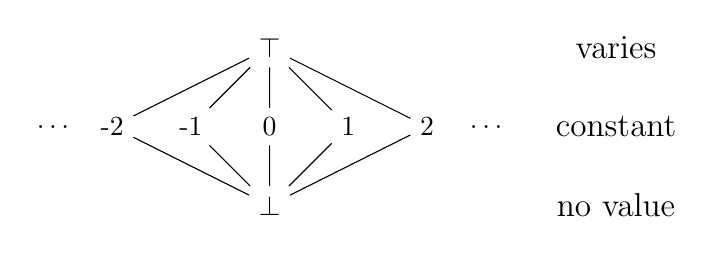
\begin{tikzpicture}[scale=1]
          \node (top)  at ( 0, 1) {$\top$};
          \node (bot)  at ( 0,-1) {$\bot$};
          \node (-3)   at (-2.75, 0) {$\hdots$};
          \node (-2)   at (-2, 0) {-2};
          \node (-1)   at (-1, 0) {-1};
          \node (0)    at ( 0, 0) {0};
          \node (1)    at ( 1, 0) {1};
          \node (2)    at ( 2, 0) {2};
          \node (3)    at ( 2.75, 0) {$\hdots$};
          %% TODO: left-align these
          \node (varying)   at (4.4, 1) {\large varies};
          \node (constant)  at (4.4, 0) {\large constant};
          \node (undefined) at (4.4,-1) {\large no value};
          \draw (bot) -- (-2) -- (top) -- (-1) -- (bot) -- (0) -- (top)
          -- (1) -- (bot) -- (2) -- (top);
        \end{tikzpicture}
      \end{center}
    \end{itemize}
  \end{frame}


  \begin{frame}
    \centering\emph{More!}
    %% \strong{Fixed points} of \strong{monotone maps} on \strong{semilattices}:
    \vspace{1ex}

    \begin{itemize}
    \item Graph algorithms
    \item Static analysis (as \emph{abstract interpretation})
    \item Typechecking
    \item Regular expression equivalence
    \item Parsing
    %% \item Logical deduction
    \end{itemize}
  \end{frame}


  \newcommand\conj{,\,}
  \begin{frame}{}
    \centering \strong{Datalog!}
    \begin{fleqn}[1em]
    \begin{minipage}[t][.35\paperheight]{\paperwidth}
      \[\begin{array}{l}
      \n{reach}(\c{start}).\\
      \n{reach}(Y) \gets \n{reach}(X)\conj \n{edge}(X,Y).\\[1ex]\pause
      \n{reach2}(\c{start}).\\
      \n{reach2}(Y) \gets \n{reach2}(X)\conj \n{edge2}(X,Y).\\[1ex]
      \n{reach3}(\c{start}).\\
      \n{reach3}(Y) \gets \n{reach3}(X)\conj \n{isnt-this-tedious}(X,Y).
      \\[1ex]
      \n{reach4}(\c{start}).\\
      \n{reach4}(Y) \gets \n{reach4}(X)\conj \n{yes-it-is-rather}(X,Y).
      \\[1ex]
      \n{reach5}(\c{start}).\\
      \n{reach5}(Y) \gets \n{reach5}(X)\conj \n{yes-it-is-rather}(X,Y).\\
      \end{array}\]
    \end{minipage}
    \end{fleqn}
  \end{frame}


  \begin{frame}
    \huge
    \begin{center}
      %\setlength\tabcolsep{1em}
      \addtolength\tabcolsep{.75ex}
      \begin{tabular}{@{}lcc@{}}
        \scshape\color{Blue} datalog
        & \color{Red!80!black} repeat yourself
        & \color{Red!80!black} sets only
        \pause
        \\
        & $\downarrow$ & $\downarrow$
        \\
        \scshape\color{Blue} datafun
        & \color{Green!80!black} functions
        & \color{Green!80!black} lattice types
      \end{tabular}
    \end{center}
  \end{frame}


  %% \begin{frame}
  %%   \interlude
  %%   \begin{center}
  %%     {\upshape\scshape iii}\\
  %%     designing datafun
  %%   \end{center}
  %% \end{frame}


  \newcommand\nodecolor[1]{{\alt<3->{\color{ForestGreen}}{}#1}}
  \newcommand\edgecolor[1]{{\alt<3->{\color{RoyalBlue}}{}#1}}

  \begin{frame}
    \centering
    \begin{fleqn}
      \textsc{datalog}
      \[\begin{array}{l}
      \n{reach}(\c{start}).\\
      \n{reach}(Y) \gets \n{reach}(X)\conj \n{edge}(X,Y).
      \end{array}
      \]
      \vspace{0pt}\pause

      \textsc{datafun}
      \[
      \begin{array}{l}
      \n{reachable} \isa
      \nodecolor{\tnode} \to
      \edgecolor{\tset{(\tnode \x \tnode)}}
      \to {\alt<4->{\mvarcolor}{}\tset \tnode}\\
      %% \n{reachable} \;\n{start} \;\n{edge} = \pause
      \n{reachable}
      \alt<3>{\hphantom{{}\isa{}}}{\;} \nodecolor{\n{start}}
      \alt<3>{\hphantom{i\to{}}}{\;} \edgecolor{\n{edge}}
      = \pause\pause
      \\\quad
      %% \eletfix{\mvar R}{\uncover<4->{\eset{\n{start}} \cup
      %%   \esetfor{y}{x \in \mvar R, (x,y) \in \n{edge}}}}
      %% \\\quad
      %% \kw{in}~\mvar R
      \efixis{\mvar R}
      \\\qquad
      \uncover<5->{\eset{\n{start}} \cup
        \esetfor{y}{x \in \mvar R, (x,y) \in \n{edge}}}
      \end{array}\]
    \end{fleqn}
  \end{frame}


  %% TODO: connect this up somehow, either arrows or hilighting in different
  %% colors.
  %\newcommand\setcolor[1]{{\alt<3->{\color{ForestGreen}}{}#1}}
  \newcommand\setcolor[1]{{\alt<3->{\color{RoyalBlue}}{}#1}}
  \newcommand\fixptcolor[1]{{\alt<4->{\mvarcolor}{}#1}}
  \newcommand\functioncolor[1]{{\alt<2->{\color{ForestGreen}}{}#1}}

  \begin{frame}
    \[
      \begin{array}{l}
      \functioncolor{\n{reachable} \;\n{start} \;\n{edge} = }
      \\\quad
      \fixptcolor{\efixis{R}}
      \\\qquad
      \setcolor{\eset{\n{start}} \cup
        \esetfor{y}{x \in \fixptcolor{R}, (x,y) \in \n{edge}}}
    \end{array}\]
      %% \[\begin{array}{l}
    %% \n{reach} \isa
    %% \tnode
    %% \to \setcolor{\tset (\tnode \x \tnode)}
    %% \to \setcolor{\tset \tnode}\\
    %% \n{reach} \;\n{start} \;\n{edge} =
    %% \fixptcolor{\kw{fix}~ {\color{black}R}~\kw{is}~}
    %% \compcolor{\{\n{start}\}
    %% \cup \setfor{y}{x \in R, (x,y) \in \n{edge}}}
    %% \end{array}\]

    \pause
    \strong{Datafun}\textsuperscript{\sffamily\scshape[icfp 2016, popl 2020]}
    is:
    \begin{itemize}\setlength\itemsep{.5ex}
    \item a \functioncolor{pure functional language} \pause
    \item with \setcolor{sets \& set/lattice comprehensions} \pause
    \item and \fixptcolor{monotone fixed points} \pause
    \item where \emph{the type system tracks monotonicity}.
    \end{itemize}
    \vspace{\baselineskip}

    %% \strong{Datafun}\textsuperscript{\sffamily\scshape[icfp 2016]} is a
    %% simply-typed \fn-calculus where \emph{types are posets} and \emph{all functions are
    %% monotone},
    %% %
    %% extended with\vspace{1ex}
    %% \begin{itemize}
    %% \item a finite set datatype \& set comprehensions;
    %% \item a bottom-up monotone fixed point operator;
    %% \item and a \emph{discreteness} comonad, $\iso$.
    %% \end{itemize}

  \end{frame}


  %% \begin{frame}
  %%   \todo{slide on types as posets, join operators?}
  %% \end{frame}

  %% \renewcommand\tset[1]{{\{#1\}}}
  %% \renewcommand\tmap[2]{{\{#1 \mapsto #2\}}}
  \newcommand\discolor{\color{RoyalBlue}}

  \begin{frame}{monotonicity types}
    %% \large
    \centering

    \setlength\tabcolsep{1em}
    \begin{tabular}{clc}
      \textbf{Type} & \textbf{Meaning} & \textbf{Ordering} %& \textbf{Join}
      \\\midrule
%        $\N$ & naturals & $0 < 1 < 2 < \hdots$ \\
      $\tbool$ & booleans & $\efalse < \etrue$ %& logical or
      \\
      $\tset A$      & finite subsets of $A$ & ${\subseteq}$ %& union
      \\
%        $\tmap A B$ & finite maps from $A$ to $B$ & \multicolumn{1}{c}{pointwise}\\
      $A \to B$   & functions & \multicolumn{1}{c}{pointwise}\\
      $A \mto B$  & \textbf{monotone} functions & \multicolumn{1}{c}{pointwise}
    \end{tabular}

    \pause
    \[\begin{array}{l}
      \n{member} \isa {\discolor \N \to{}} {\mvarcolor\tset{\N} \mto{}} \tbool\\
      \n{member}\; {\discolor x}\; \mvar{S} = \exists({\discolor y} \in \mvar{S})\;
      {\discolor x} = {\discolor y}
    \end{array}\]

    \pause
    \pbox{.8\textwidth}{
    variables are \emph{discrete} {\discolor $x,y,z$}\\
    \phantom{variables are }\hspace{-2.28em}or \emph{monotone}
    {\mvarcolor $X,Y,Z$}
    }

  \end{frame}


  %% \begin{frame}{monotonicity}
  %%   \centering

  %%   {\small\todo{line up types with arguments}
  %%   \todo{emphasize plus over arrow}
  %%   \todo{colors for disc/mono?}}

  %%   \[
  %%   \begin{array}{l}
  %%     \n{member} \isa \N \to \tset{\N} \mto \tbool\\
  %%     \n{member} \;x \;S =
  %%     \exists (y \in S)\; {x = y}
  %%   \end{array}
  %%   \]
  %%   \vspace{.4em}\pause

  %%   \pbox{.8\textwidth}{
  %%   functions are
  %%   \emph{discrete} $A \to B$\\
  %%   \phantom{functions are }\hspace{-2.005em}or \emph{monotone} $A \mto B$
  %%   }
  %%   \vspace{1.5em}\pause

  %%   \pbox{.8\textwidth}{
  %%   variables are \emph{discrete} $x,y,z$\\
  %%   \phantom{variables are }\hspace{-2.005em}or \emph{monotone} $X,Y,Z$
  %%   }

  %%   %% \pbox{.8\textwidth}{
  %%   %% functions are
  %%   %% \emph{discrete} $A \to B$\\
  %%   %% \phantom{functions are }\hspace{-2.005em}or \emph{monotone} $A \mto B$
  %%   %% \\[1em]
  %%   %% variables are \emph{discrete} $x,y,z$\\
  %%   %% \phantom{variables are }\hspace{-2.005em}or \emph{monotone} $X,Y,Z$
  %%   %% }

  %%   %% \setlength\tabcolsep{0pt}
  %%   %% \begin{tabular}{r@{\qquad}rl}
  %%   %%   functions are \emph{discrete} $A \to B$
  %%   %%   & variables are \emph{discrete} &\ $x,y,z$\\
  %%   %%   or \emph{monotone} $A \mto B$
  %%   %%   & or \emph{monotone} &\ $X,Y,Z$
  %%   %% \end{tabular}

  %% \end{frame}


  \begin{frame}{lattice comprehensions}
    How does this expression \emph{run}?
%
    \[
    \def\arraystretch{1.33}
    \begin{array}{rl@{\hspace{6em}}}
      &\esetfor{x + 1}{x \in \eset{2,3}}
      \\\pause
      \desugars& \eforvar{x}{\eset{2,3}} \eset{x + 1}
      \\\pause
      \text{\small (which is a big semilattice join:)}& \displaystyle\bigsqcup_{x \in \eset{2,3}} \eset{x + 1}
      \\\pause
      =& \eset{2 + 1} \cup \eset{3 + 1}
      \\
      =& \eset{3,4}
    \end{array}\]
  \end{frame}

  \begin{frame}{lattice comprehensions}
    \[
    \exists (y \in S)\; x = y
    \pause\,\desugars\,
    \eforvar{y}{S} x = y
    \]
    %% \[
    %% \def\arraystretch{1.33}
    %% %\begin{aligned}
    %%   \begin{array}{cl}
    %%     &\exists (y \in S)\; {x = y}\\\pause
    %%     =& \eforvar{y}{S} {x = y}
    %%     %\\ =& \displaystyle\bigvee_{y \in S} {x = y}
    %%   \end{array}
    %% %\end{aligned}
    %% \]

    \pause
    \[
    \def\arraystretch{1}
    \begin{array}{rl}
      &\setfor{y}{x \in R, (x,y) \in \n{edge}}\\\pause
      \desugars&
      \eforloop{x \in R}
      \\& \quad
      \eforloop{(x,y) \in \n{edge}}
      \\& \qquad
      \eforjoin \eset{y}
      \\\pause
      \desugars&
      \eforloop{x_1 \in R}\\
      &\quad \eforloop{(x_2,y) \in \n{edge}}
      \\&\qquad
      \eforwhen{x_1 = x_2} \eforjoin \eset{y}
    \end{array}
    \]
    %% How about these?
    %% %
    %% \begin{mathpar}
    %%   \exists (y \in S)\; {x = y}

    %%   \setfor{y}{x \in R, (x,y) \in \n{edge}}
    %% \end{mathpar}
  \end{frame}


  \begin{frame}{fixed points}
    %% \todo{return to transitive closure?}
    %% \todo{then move on to shortest path?}

    \[\begin{array}{l}
    %\n{reach} \isa \tnode \to \tset{(\tnode \x \tnode)} \to \tset \tnode\\
    \n{reachable} \;\n{start} \;\n{edge} = \efixis{{\standout R}}
    \{\n{start}\} \cup \setfor{y}{x \in {\standout R}, (x,y) \in \n{edge}}
    \\[1em]\pause
    \n{shortest} \isa \tnode \to \tset{(\tnode \x \tnode \x \tpname{dist})}
    \to \tmap{\tnode}{\tpname{dist}}
    \\
    \n{shortest} \;\n{start} \;\n{edge} =
    \\\quad
    \efixis{\mvar M}
    \\\qquad
    \phantom{\sqcup{}}
    \eset{\n{start} \mapsto \text{\liningnums{0}}}
    %\sqcup {}
    \\
    %\phantom{\n{shortest} \;\n{start} \;\n{edge} =}{}
    \qquad
    \sqcup
    \esetfor{y \mapsto \mvar{D_1} + d_2}
            {(x \mapsto \mvar{D_1}) \in \mvar M, (x,y,d_2) \in \n{edge}}
    \end{array}
    \]
  \end{frame}


  %% \begin{frame}{cyk parsing}
  %%   \todo{CYK parsing example goes here}
  %% \end{frame}


  \begin{frame}
    \interlude
    \begin{center}
      {\upshape\scshape iv}
      \\
%      semi\naive\ evaluation\\
      deltas \emph{\&} derivatives
    \end{center}
  \end{frame}


  \begin{frame}
    \[\n{step}\;R =
    {\color<-2>{RoyalBlue}\{\n{start}\}}
    \cup
    {\color<-2>{Red}\setfor{y}{x \in R, (x,y) \in \n{edge}}}
    \]

    \pause\begin{align*}
      R_0 &= \emptyset
      & \uncover<3->{dR_0} &\uncover<3->{= }\uncover<4->{\color<-5>{RoyalBlue}\{\n{start}\}}
      \\
      R_{i+1} &= \makebox[4.3em][l]{$\alt<6->{\hi{R_i \cup dR_i}}{\n{step}\;R_i}$}
      & \uncover<3->{dR_{i+1}} &\uncover<3->{= }\uncover<5->{\color<-5>{Red} \setfor{y}{x \in dR_i, (x,y) \in \n{edge}}}
    \end{align*}

    \centering\alt<3->{
      \includegraphics[height=45mm]{imgs/focus-1240.jpg}
    }{
      \includegraphics[height=45mm]{imgs/focus-0946.jpg}
    }
    \vspace{1ex}
  \end{frame}


  \begin{frame}{}{}\huge\centering
    \setlength\parskip{2ex}

    {\scshape semi\naive\ evaluation}

    means

    %% {\bf computing the changes between iterations}
    {computing the {\strong{changes}} between iterations}

    %% {by}
    %% {\bfseries incrementalizing the step function}
  \end{frame}


  %% \newcommand\chgto\rightsquigarrow
  %% \newcommand\chgat[4]{{\ensuremath{{#2} \dblcolon_{#1} {#3} \chgto {#4}}}}
  %% \newcommand\chg[3]{{\ensuremath{{#1} \dblcolon {#2} \chgto {#3}}}}

  %% \begin{frame}{Incremental \fn-calculus
  %%     \textsuperscript{\sffamily[%
  %%         Cai et al \textsc{pldi 2014},
  %%         Giarrusso's thesis \textsc{2017},
  %%         Giarrusso et al \textsc{esop 2019}]}}
  %%   Every type $A$ has a \emph{change type} $\D A$ and a relation
  %%   $\chgat{A}{dx}{x}{y}$, where $x,y : A$ and $dx : \D A$.

  %%   \vspace{1ex}
  %%   \setlength\arraycolsep{.2em}
  %%   \[
  %%   \begin{array}{rcl@{\qquad}c}
  %%     \D(\tset A) &=& \tset A & \chgat{\tset A}{dx}{x}{x \cup dx}
  %%     \\[1.5ex]\pause
  %%     \D(A \x B) &=& \D A \x \D B &
  %%     \infer{\chgat A{da} a {a'} \\ \chgat B{db} b {b'}
  %%     }{\chgat{A \x B}{(da,db)}{(a,b)}{(a',b')}}
  %%     \\[3.5ex]\pause
  %%     \D(\iso A) &=& \tunit & \chgat{\iso A}{()}{x}{x}
  %%   \end{array}
  %%   \]
  %% \end{frame}

  %% \newcommand\underexplain[4]{%
  %%   \underaccent{%
  %%     \parbox[t][#1]{#2}{\sffamily\centering\vspace{4pt}\small#3}
  %%   }{#4}}

  %% \newcommand\chgatcov[4]{{\uncover<2->{{#2} \dblcolon_{#1}} {#3} \chgto {#4}}}
  %% %\newcommand\chgatcovb[4]{{\uncover<5->{{#2} \dblcolon_{#1}} {#3} \to {#4}}}
  %% \begin{frame}\LARGE
  %%   %\setbeamercovered{transparent}

  %%   \begin{mathpar}
  %%     \D(A \mto B)
  %%     = \underexplain{}{1.5cm}{original input}{A}
  %%     \to \underexplain{}{1.2cm}{change to input}{\D A}
  %%     \mto \underexplain{}{1.4cm}{change in output}{\D B}
  %%     \\\pause
  %%     \chgat{A \mto B}{df}{f}{\alt<5->{\hi f}{g}} \iff \pause
  %%     \infer{\chgat{A}{dx}{x}{y}
  %%     }{\chgat{B}{\uncover<4->{df\;x\;dx}}{f\;x}{\alt<5->{\hi f}{g}\;y}}
  %%     %% \infer{\chgatcov{A \to B}{df}{f}{\alt<3>{\hi{f}}{g}}\\
  %%     %%   \chgatcov{A}{dx}{x}{y}
  %%     %% }{
  %%     %%   \chgatcov{B}{df\;x\;dx}{f\;x}{\alt<3>{\hi f}{g}\;y}
  %%     %% }
  %%   \end{mathpar}

  %%   \setbeamercovered{invisible}
  %%   \vspace{2ex}\centering\pause\pause
  %%   In this case, we call $df$ the
  %%   \strong{derivative} of $f$.

  %%   \vspace{\baselineskip}

  %%   %% \[
  %%   %% \infer{
  %%   %%   \fa{\chgat A {dx} x y}\, \chgat B {df\;x\;dx} {f\;x} {g\;y}
  %%   %% }{\chgat{A \to B}{df} f g}
  %%   %% \]
  %% \end{frame}


  \begin{frame}%{change in datafun}
    \setlength\parskip{1ex}

    Every type $A$ gets a type $\standout\Delta A$ of \emph{increasing} changes,
    e.g.
    %
    \begin{mathpar}
      \Delta(\tset{A}) = \tset{A}
      %% \Delta(A \x B) = \Delta A \x \Delta B
    \end{mathpar}

    \pause
    To incrementalize, we \emph{push changes through the program},
    finding the change $\standout\delta(e)$ to an expression, e.g.
    %
    \begin{mathpar}
      \delta(s \cup t) = ds \cup dt

      \delta(s \setminus t) = ds \setminus t
      %\pause{\delta(\n{size} \;s) = \n{size} \;(s \cup ds)}
      \\%\pause
      \standout
      %% \delta(\fnof{X} e)?
      \delta(\eforvar{x}{s} e)?
    \end{mathpar}
    %% \begin{align*}
    %%   \delta(s \cup t) &= ds \cup dt\\
    %%   \uncover<3->{\delta(s \setminus t) &= ds \setminus t}
    %%   \\
    %%   \uncover<4->{\delta(\n{size} \;s) &= \n{size} \;(s \cup ds)}
    %% \end{align*}
  \end{frame}


  \begin{frame}
    \begin{align*}
      \delta(\eforvar{x}{s}{e})
      &=
      \phantom{{}\join{}}
      (\eforvar x {ds} e)
      \\
      &\phantom{{}={}} {}\join
      (\eforvar x {s \cup ds}
      %\elet{dx = \zero \;x}
      \delta(e))
    \end{align*}

    \todo{have a concrete example?}
  \end{frame}


  \begin{frame}
    \strong{Ideas to take away:}\vspace{1ex}
    \begin{itemize}
    \item Bottom-up monotone fixed points are neat.

      {\normalsize \textbf{applications}: \itshape static analysis, parsing,
        shortest paths, regular expression matching}

    \item To compute them efficiently, \emph{incrementalize the inner loop} by
      propagating changes through your program.

    \item Types let us control what things we need to incrementalize!
    \end{itemize}
    \vspace{\baselineskip}
  \end{frame}


  \begin{frame}
    \centering
    {\scshape future and related work}

    \begin{itemize}
      \setlength\itemsep{2ex}
    \item \emph{Efficiency!} via... %\vspace{1ex}

      \begin{center}
        \large
        \begin{tabular}{ccc}
          \emph{\normalsize imitating Datalog:}
          &
          \emph{\normalsize compiling to Datalog:}
          &
          \emph{\normalsize emitting Datalog:}
          \\
          query optimization?
          & query normalization?
          & staged computation?
        \end{tabular}
      \end{center}

    \item Custom semilattice types / deltas via SMT?
      \\
      {\large\itshape see {\upshape\scshape Flix}}

    \item Concurrent and/or distributed computation?
      \\
      {\large\itshape see LVars, CALM}

      \item Incrementalize fixed point maintenance?
        \\
        {\large\itshape see Differential Dataflow, Mario Picallo's thesis}
    \end{itemize}

    %% \todo{{RETROSPECTIVE:} Datafun is neat, but it took a lot of work to
    %%   generalize seminaive evaluation to handle higher-order functions, and
    %%   would need significantly more work to make Datafun efficient by porting
    %%   over query optimisation, etc. Not clear the added complexity is worth it
    %%   as a way of making datalog more expressive; power-to-weight ratio, etc. If
    %%   I did it again, might try staged computation - separate flexible
    %%   higher-order bit from highly optimisable first-order bit.}
  \end{frame}


  \appendix
  \begin{frame}
    \centering\Huge\displayfamily
    \color{gray!10}\itshape%
    un{\upshape\scshape\color{black}\standout fin}%
    \color{gray!10}ished
  \end{frame}


  \begin{frame}
    \todo{BACKUP SLIDES:}
    \begin{itemize}
    \item delta for functions
    \item the box type
    \item concurrency graphs
    \end{itemize}
  \end{frame}

\end{document}
